\documentclass[11pt]{article} % 
\usepackage[pdftex]{graphicx}
\usepackage{fullpage}
\usepackage{graphicx}
\usepackage{graphics}
\usepackage{psfrag}
\usepackage{pgf}
\usepackage{color}
\usepackage{tikz}
\usepackage{epstopdf}
\usetikzlibrary{arrows,automata}
\usepackage[latin1]{inputenc}
\usepackage{amsthm}
\usepackage{amsmath,amssymb}
\usepackage{enumerate}
\setlength{\textwidth}{6.5in}
\setlength{\textheight}{9in}
\newcommand{\N}{\mathbb{N}}
\newcommand{\Z}{\mathbb{Z}}
\newcommand{\R}{\mathbb{R}}
\newcommand{\Q}{\mathbb{Q}}
\newcommand{\C}{\mathbb{C}}
\newcommand{\PP}{\mathbb{P}}
\newcommand{\tab}{\;\;\;\;\;}
\newcommand{\inv}{^{-1}}
\newcommand{\tr}{\textrm}
\newcommand{\lc}{\sqcup}
\newcommand{\var}{\tr{Var}}
\newcommand{\cov}{\tr{Cov}}
\newcommand{\like}{\mathcal{L}}

\begin{document}

\hfill Blace Houle \& Robert Johns

\hfill April 17, 2014

\begin{center} {\Large CSCI 678: Statistical Analysis of Simulation Models}\\{\large Homework 11}\end{center}

\begin{enumerate}

%1
\item The average time in the system for a customer is $E[T] = E[W] + E[S]$, where $W$ is the time waiting and $S$ is the time in service.  We see that $E[S]$ is the mean of a $U(1,2)$ process, which is $1.5$, and $V[S] = 1/12$.  We can further break down $E[W]$ into $E[n] * E[S] + E[r]$, where $n$ is the number of customers in line ahead of the arrival, $E[S] = 1.5$ as previously found, and $E[r]$ is the expected time remaining on the job being processed when the customer arrives.  The solving for $E[n]$ and $E[r]$ is a long and arduous process, but after much wailing and gnashing of teeth (internet searching), we get that
$$E[T] = E[S]\left[\frac{1 + V[S]/E[S]^2}{2} * \frac{\lambda/\mu}{1 - \lambda/\mu} + 1\right]$$
plugging in our known values, we get that
$$E[T] = 3.8333...$$

%%%%%
%2
\item $$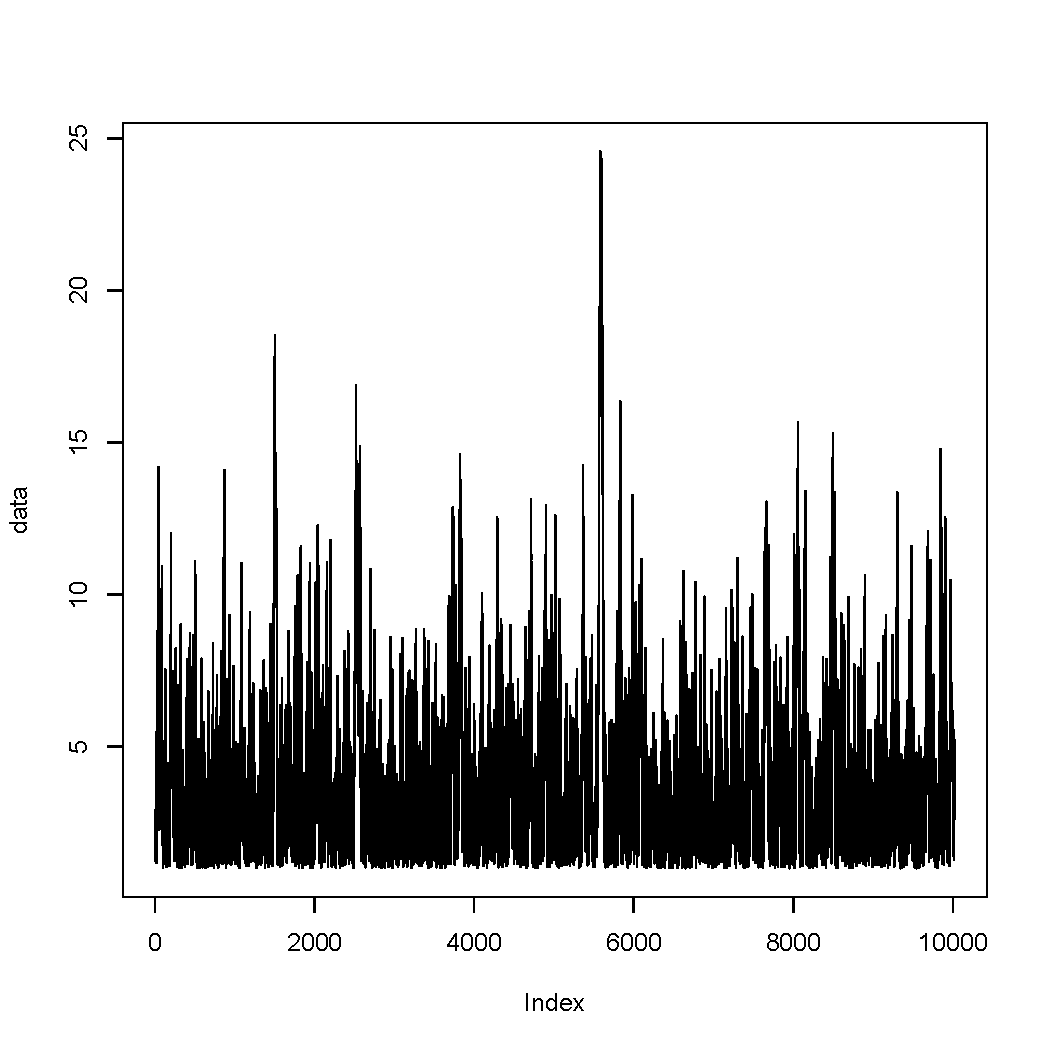
\includegraphics[scale = .75]{plot1.pdf}$$

%%%%%
%3
\item $${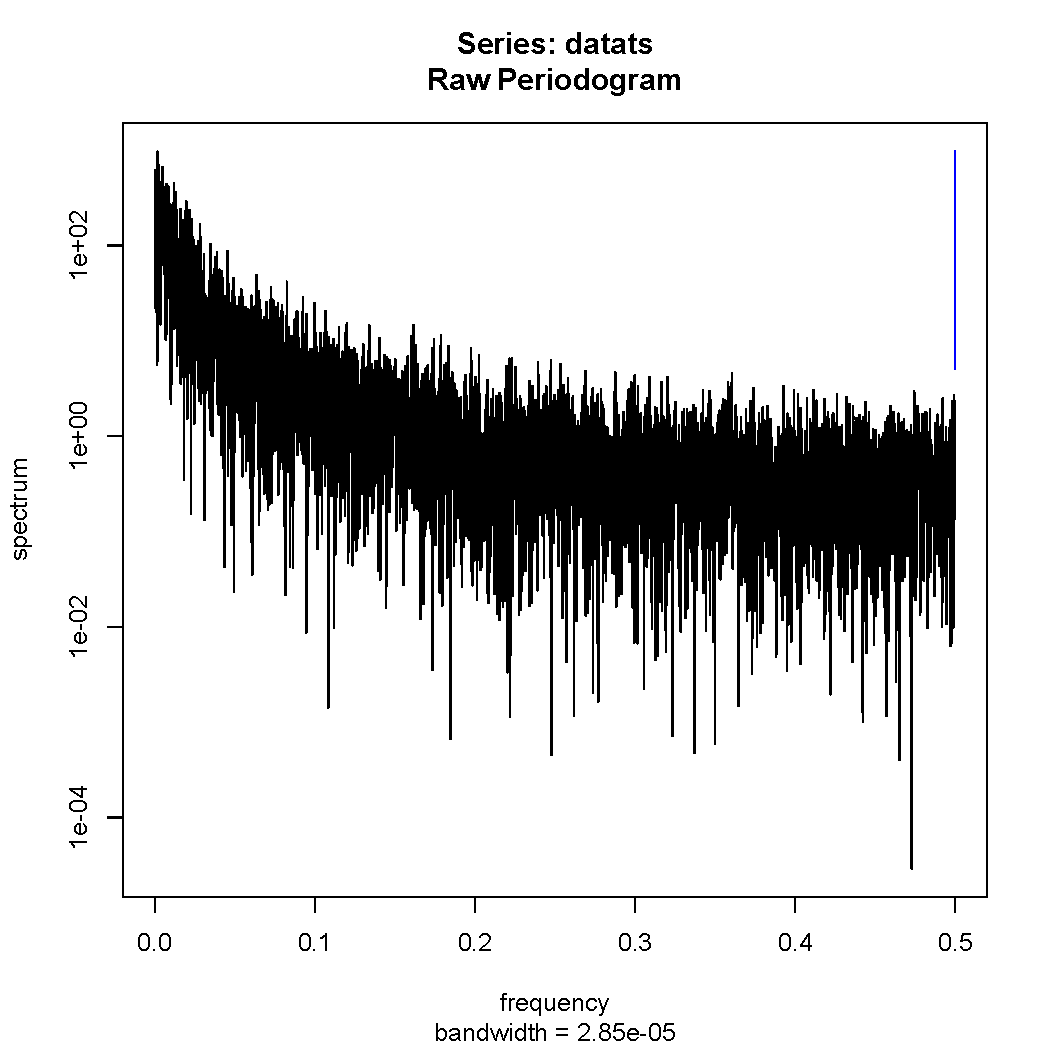
\includegraphics[scale = .5]{plot2.pdf}}$$

We see a constant downward trend that levels off around .2.  The height around lower frequencies tells us that the data is more correlated with longer periods; that is, the cyclic trend in the time series is rather long.  When examining the data, this seems logical; we see regular periodic spikes every 5000 observations or so.  The leveling off around .2 tells us that frequencies greater than .2 contribute equally to correlation. (Note: it's hard to tell the real periodic nature from the graph of wait times, because it's so dense and we don't know how to manipulate axes in R).

%%%%%
%4
\item The program \texttt{asm11a.c} (attached at end) was used to find the confidence intervals.  It's results are printed below:

\begin{verbatim}(i)   Classic Confidence Interval:
      (3.503734,4.329389)

(ii)  Nonoverlapping Batch Mean interval:
      (3.674883,4.158240)

(iii) Overlapping Batch Mean interval:
      (3.656754,4.176369)

(vii) Standardized Time Series interval:
      (3.909522,3.923601)

mean wait: 3.916562\end{verbatim}

\end{enumerate}

\end{document}